\documentclass{article}
\usepackage{amsmath}
\usepackage{array}
\usepackage{color}
\usepackage{graphicx}
\usepackage{float} %utiliser H pour forcer � mettre l'image o� on veut
\usepackage{lscape} %utilisation du mode paysage
\usepackage{mathbbol} % permet d'avoir le vrai symbol pour les reels grace a mathbb
\usepackage{enumerate}
\usepackage{marvosym}	
\usepackage{moreverb} % permet d'utiliser verbatimtab : conservation la tabulation 


\setlength {\textwidth}{16cm}
\setlength {\textheight}{21cm} 
\setlength {\oddsidemargin}{0cm}
\setlength{\headsep}{5pt} 

\newcommand\bn{\boldsymbol{\nabla}}
\newcommand\bo{\boldsymbol{\Omega}}
\newcommand\br{\mathbf{r}}
\newcommand\la{\left\langle}
\newcommand\ra{\right\rangle}
\newcommand\bs{\boldsymbol}

\renewcommand{\(}{\left(}
\renewcommand{\)}{\right)}
\renewcommand{\[}{\left[}
\renewcommand{\]}{\right]}

\newtheorem{theorem}{Theorem}[section]

\begin{document}
\title{\textsc{\huge{Optimization methods}}}
\author{Bruno Turcksin} 
\date{}
\maketitle

\section{Types of optimization}
We can write the optimization problem as :
\begin{description}
\item [Linear optimization :] all functions are linear
\item [Global optimization :] the objective function has multiple local minimizers
\item [Convex feasibility problem :] no objective function, only constraints to respect
\item [Multi-objective optimization :] the problem has more than one objective function
\end{description}

\subsection{Linear optimization}
We can use the following methods to solve them :
\begin{enumerate}
\item Simplex algorithm.
\item Interior point methods. Faster than the simplex if :
\begin{itemize}
\item problem is degenerate
\item no good initial guess is available
\item number of constrains is very large
\item matrix $A$ is not sparse ($Ax=b$)
\end{itemize}
\end{enumerate}
Advantages of this formulation :
\begin{itemize}
\item Only 1 minimum
\end{itemize}
Disadvantages of this formulation :
\begin{itemize}
\item Time to solve the problem can be very long
\item Mixed integer programming needed to handle dose-volume constraint
\end{itemize}

\subsection{Global optimization}
We can use the following methods to solve them :
\begin{enumerate}
\item Simulated Annealing (stochastic) :
\begin{itemize}
\item we will find the global minimum, if we have the time
\end{itemize}
\item Lipschitz method (deterministic) :
\end{enumerate}

\subsection{Convex feasibility problem}
We can use the following methods to solve them :
\begin{enumerate}
\item POCS algorithm :
\begin{equation}
x^{k+1} = x^k + \lambda_k \(P_{\bot_{j(k)}}\(x^k\)-x^k\)
\end{equation}
\item Cimmino's algorithm :
\begin{equation}
x^{k+1} = x^k + \lambda_k \(\sum_{j=1}^J w_j P_{\bot_{j(k)}}\(x^k\)-x^k\)
\end{equation}
\item Cyclic Subgradients Projections (CSP) and Simultaneous Subgradients Projections (SSP)
\end{enumerate}

\subsection{Multi-objective function}
We can use the following methods to solve them :
\begin{enumerate}
\item Scalarization : 
\begin{itemize}
\item conversion of the multi-objective problem into a scalar optimization problem. Problem find the weight (see our code)
\end{itemize}
\item Pareto optimality (course of ULB)
\end{enumerate}

\subsection{Gradient method}
We can use the following methods to solve them :
\begin{enumerate}
\item Newton's
\item Steepest descent
\item Gauss-Newton
\item ...
\end{enumerate}

\section{Deterministic algorithm}
\subsection{Core algorithm}
$x$ = input and $z$ = outcome, ($z=\phi(x)$)
\begin{itemize}
\item Step 1 : renumber the points :
\begin{equation}
a=x_0 <x_1<\ldots<x_k=b
\end{equation}
\item Step 2 : compute the maximal slope :
\begin{equation}
\begin{split}
M &= \max_{1\leq i\leq k} \left| \frac{z_i - z_{i-1}}{x_i -x_{i-1}} \right|\\
&= \max\(M_{k-1},\frac{|z_{k+1}-z_{t-1}|}{x_{k+1}-x_{t-1}},\frac{|z_{t}-z_{k+1}|}{x_{t}-x_{k+1}}\)
\end{split}
\end{equation}
\item Step 3 : Accept the estimate :
\begin{equation}
m =\left\{
\begin{aligned}
1, &\ M=0\\
rM, &\ M>0
\end{aligned}
\right.
\end{equation}
where $r>1$ is the input of the algorithm.\\
\item Step 4 : for each interval $(x_{i-1},x_i)$, $1\leq i \leq k$, calculate the value :
\begin{equation}
R(i) = m(x_i - x_{i-1}) + \frac{(z_i-z_{i-1})^2}{m(x_i-x_{i-1})}-2(z_i + z_{i-1})
\end{equation}
called characteristic of the interval.
\item Step 5 : Select the interval $(x_{t-1},x_t)$ corresponding to the maximal characteristic :
\begin{equation}
R(t) = \max_{i\leq i \leq k} R(i)
\end{equation} 
if there is more than 1 solution, take the smaller integer
\item Step 6 : Accept :
\begin{equation}
x^{k+1} = \frac{x_t+x_{t-1}}{2} - \frac{z_t - z_{t-1}}{2m}
\end{equation}
\end{itemize}
Variants :
\begin{itemize}
\item Possibility to handle discontinuous function if the global minimum is not on the discontinuity. Might be necessary to change the mapping. 
\item Global Search Mixed Algorithm (p202)\footnote{Global optimization with non-convex constraints} : uses a local refinement to check some interesting vicinity.
\item Local tuning of the Lipschitz method (p236) : if there is a region where $L$ is large, it does not slow down the search in the region where $L$ is small. This is very important to do! We can also use better auxiliary functions than the piecewise-linear
\item We can use higher order functions to approximate the function :
\begin{itemize}
\item Step 1 : renumber the points :
\begin{equation}
a=x_0 <x_1<\ldots<x_k=b
\end{equation}
\item Step 2 : compute the maximal slope :
\begin{equation}
M = \max\{m_i:1<i\leq k\}
\end{equation}
where :
\begin{equation}
m_i = \max
\left\{
\begin{aligned}
&\frac{|z_i'-z_{i-1}'|}{x_i-x_{i-1}}\\
&2\frac{-z_i+z_{i-1}+z_{i-1}'(x_i-x_{i-1})}{(x_i-x_{i-1})^2}\\
&2\frac{z_i-z_{i-1}-z_i'\(x_i-x_{i-1}\)}{(x_i-x_{i-1})^2}
\end{aligned}
\right.
\end{equation}
where $z_i=\phi(x_i)$ and $z_i'=\Phi'(x_i)$
\item Step 3 : Accept the estimate :
\begin{equation}
m =\left\{
\begin{aligned}
1, &\ M=0\\
rM, &\ M>0
\end{aligned}
\right.
\end{equation}
where $r>1$ is the input of the algorithm.\\
\item Step 4 : for each interval $(x_{i-1},x_i)$, $1\leq i \leq k$, calculate the value :
\begin{equation}
R(i) = z_{i-1} + z_{i-1}'(\hat{x}_i - x_{i-1}) -0.5m\(\hat{x}-x_{i-1}\)^2
\end{equation}
called characteristic of the interval and where :
\begin{equation}
\hat{x}_i=\frac{-z_i+z_{i-1}+z_i'x_i-z_{i-1}'x_{i-1}+0.5m\(x_i^2-x_{i-1}^2\)^2}{m\(x_i-x_{i-1}\)+z_i'-z_{i-1}'} \label{x_hat}
\end{equation}
\item Step 5 : Select the interval $(x_{t-1},x_t)$ corresponding to the maximal characteristic :
\begin{equation}
R(t) = \max_{i\leq i \leq k} R(i)
\end{equation} 
if there is more than 1 solution, take the smaller integer
\item Step 6 : Accept :
\begin{equation}
x^{k+1} = \hat{x}_t
\end{equation}
where $\hat{x}_t$ is calculated according to (\ref{x_hat})
\item We can do the local tuning here also.
\end{itemize}
The method is better when we use a smooth approximation.
\item When we have several processors (p) available, we try on p intervals $\Longrightarrow$ not very efficient with a lot of processors.
\end{itemize}
Example : The function to minimize is :
\begin{equation}
y = (10x)^2 + 10 \sin(1000x)
\end{equation}
The objective function looks like :
\begin{figure}[H]
\centering
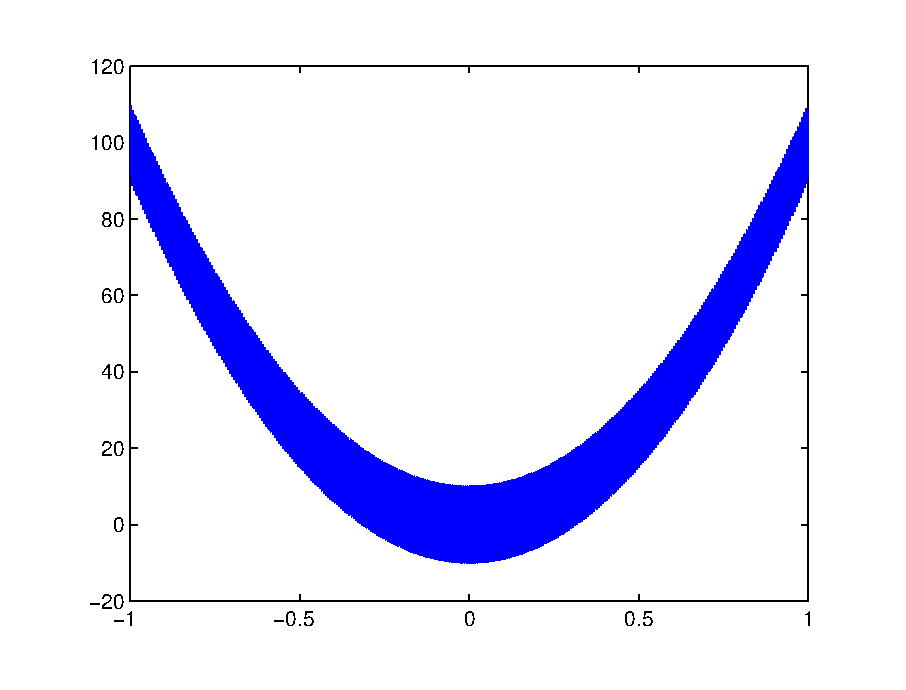
\includegraphics[width=9cm]{GSA}
\end{figure}
The minimum is in 0 where the objective function is -9.99975 around -0.00157. The value given by GSA is -9.902866 in 0.02365. It took 468 iterations and 0.4065 seconds (tolerance = $10^{-3}$). The value given by GSA is -9.8463206 in 0.0171. It took 95 iterations and 0.021353 seconds (tolerance = $10^{-2}$). As we can see, we did not find the global minimum. However, the difference of the objective function between the minimum found by GSA and the global minimum is less than 1\%.

\section{Dose-volume constraints}
% to do
\end{document}
